\chapter{Material models}
\label{matmodels}

%%%%%%%%%%%%%%%%%%%%%%%%%%%%%%%%%%%%%%%%%%%%%%%%%%%%%%%%
%%%%%%%%%%%%%%%%%%%%%%%%%%%%%%%%%%%%%%%%%%%%%%%%%%%%%%%%
\section{General strategy}

Transport processes are based on gradients of suitable variables and on fluxes of mentioned variables.
Connection between gradients and fluxes guarantees constitutive laws. Consider transport of one medium,
e.g. heat. Basic variable is temperature. Gradient of temperature is denoted
\begin{equation}
\mbf{g} = {\rm grad}\ T = \left(\ppd{T}{x},\ \ppd{T}{y},\ \ppd{T}{z}\right)^T\ , \ \ \ \ \
g_i = \ppd{T}{x_i}\ .
\end{equation}
Flux of heat is defined by Fourier's law
\begin{equation}
\mbf{q} = \mbf{D} \mbf{g}\ ,\ \ \ \ \ \
q_i = D_{ij} g_j\ ,
\end{equation}
where $\mbf{D}$ denotes matrix of material coefficients. The simplest Fourier's law uses diagonal matrix $\mbf{D}$
where conduction coefficients are located on the diagonal.
Flux of any quantity is used in conservation law which has form
\begin{equation}
{\rm div} \mbf{q} = 0\ ,\ \ \ \ \ \
\ppd{q_i}{x_i} = 0\ .
\end{equation}

Previously described strategy is valid when one medium is transported. In case of several, say $n$, transported media,
the situation is more complicated. Each of $n$ media has its own macroscopic quantity which defines state of the medium
and is denoted as $f_i$. Gradient of each quantity can be computed and is denoted as
\begin{equation}
\mbf{g}^i = {\rm grad}\ f_i\ ,\ \ \ \ \ \
g_j^i = \ppd{f_i}{x_j}\ .
\end{equation}
Superscript denotes the quantity and subscript denotes the component.
Fluxes of particular quantities are linear combinations of gradients multiplied by material coefficients.
They can be expressed as
\begin{equation}
\mbf{q}^i = \sum_{j=1}^n \mbf{D}_j^i \mbf{g}^j\ ,\ \ \ \ \
q_j^i = D_{jk}^m g_k^m\ .
\end{equation}
The constitutive matrix $\mbf{D}_j^i$ defines interaction between the $i$-th flux and the $j$-th gradient.


%%%%%%%%%%%%%%%%%%%%%%%%%%%%%%%%%%%%%%%%%%%%%%%%%%%%%%%%
%%%%%%%%%%%%%%%%%%%%%%%%%%%%%%%%%%%%%%%%%%%%%%%%%%%%%%%%
\section{Media transfer}
%%%%%%%%%%%%%%%%%%%%%%%%%%%%%%%%%%%%%%%%%%%%%%%%%%%%%%%%

\subsection{One medium transfer}
\label{onemedtrans}
{\bf System of equations:}

\begin{eqnarray}\label{onemed}
\tenss{K}_{11}\tenss{r}_1 + \tenss{C}_{11}\dot{\tenss{r}}_1 = {\tenss{q}}_1
\end{eqnarray}

%%%%%%%%%%%%%%%%%%%%%%%%%%%%%%%%%%%%%%%%%%%%%%%%%%%%%%%%
\subsection{Two media transfer}

{\bf System of equations:}

\begin{eqnarray}
\left[ \begin{array}{cc}
\tenss{K}_{11} & \tenss{K}_{12} \\
\tenss{K}_{21} & \tenss{K}_{22}
\end{array} \right]
\left\{ \begin{array}{c}
\tenss{r}_1 \\
\tenss{r}_{2}
\end{array} \right\} + 
\left[ \begin{array}{cc}
\tenss{C}_{11} & \tenss{C}_{12} \\
\tenss{C}_{21} & \tenss{C}_{22}
\end{array} \right]
\left\{ \begin{array}{c}
\dot{\tenss{r}}_1 \\
\dot{\tenss{r}}_{1}
\end{array} \right\} = 
\left\{ \begin{array}{c}
\tenss{q}_{1} \\
\tenss{q}_{2}
\end{array} \right\}.
\end{eqnarray}

%%%%%%%%%%%%%%%%%%%%%%%%%%%%%%%%%%%%%%%%%%%%%%%%%%%%%%%%
\subsection{Three media transfer}

{\bf System of equations:}

\begin{eqnarray}
\left[ \begin{array}{ccc}
\tenss{K}_{11} & \tenss{K}_{12} & \tenss{K}_{13} \\
\tenss{K}_{21} & \tenss{K}_{22} & \tenss{K}_{23} \\
\tenss{K}_{31} & \tenss{K}_{32} & \tenss{K}_{33}
\end{array} \right]
\left\{ \begin{array}{c}
\tenss{r}_1 \\
\tenss{r}_2 \\
\tenss{r}_3
\end{array} \right\} + 
\left[ \begin{array}{ccc}
\tenss{C}_{11} & \tenss{C}_{12} & \tenss{C}_{13} \\
\tenss{C}_{21} & \tenss{C}_{22} & \tenss{C}_{23} \\
\tenss{C}_{31} & \tenss{C}_{32} & \tenss{C}_{33}
\end{array} \right]
\left\{ \begin{array}{c}
\dot{\tenss{r}}_1 \\
\dot{\tenss{r}}_2 \\
\dot{\tenss{r}}_3
\end{array} \right\} = 
\left\{ \begin{array}{c}
\tenss{q}_1 \\
\tenss{q}_2 \\
\tenss{q}_3
\end{array} \right\}.
\end{eqnarray}



%%%%%%%%%%%%%%%%%%%%%%%%%%%%%%%%%%%%%%%%%%%%%%%%%%%%%%%%
%%%%%%%%%%%%%%%%%%%%%%%%%%%%%%%%%%%%%%%%%%%%%%%%%%%%%%%%
\section{List of material models}
{\bf List of implemented models for heat and moisture transfer}

\begin{itemize}
\item{\bf isotransmat}\\ 
- calculates properties of general isotropic material for linear one medium heat or moisture transfer 
(constant conductivity/permeability and capacity)

\begin{center}
\begin{tabular}{|l|l|}
\hline
location & /TRFEL/SRC/isotrmat.cpp\\
         & /TRFEL/SRC/isotrmat.h
\\ \hline
related files &
\\ \hline
notes & 
\\ \hline
\end{tabular}
\end{center}

\item{\bf cernyconcrete}\\ 
- computes conductivity and capacity coefficients for fiber concrete for one medium heat transfer (one medium, $t$ ... temperature [$^\circ$C])\\
- data measured in the laboratory of the Department of Physics of the Faculty of Civil Engineering CTU Prague

\begin{center}
\begin{tabular}{|l|l|}
\hline
location & /TRFEL/SRC/cerny\_concrete.cpp\\
         & /TRFEL/SRC/cerny\_concrete.h
\\ \hline
related files &
\\ \hline
notes & 
\\ \hline
\end{tabular}
\end{center}

\item{\bf bazantpedersen}\\ 
- computes conductivity and capacity matrices general material for two media coupled heat and moisture transfer (two media - $w$ ... water content [kg/kg], $t$ ... temperature [K])\\
- the theory is based on Lewis' and Schrefler's theory - theory of multi-phase porous medium\\
- water vapor permeability is from Bazant and Najjar (1972)~\cite{bazant_n}\\
- sorption isotherm and hydraulic conductivity is from Pedersen (1990)~\cite{pedersen}

\begin{center}
\begin{tabular}{|l|l|}
\hline
location & /TRFEL/SRC/bazped.cpp\\
         & /TRFEL/SRC/bazped.h
\\ \hline
related files &
\\ \hline
notes & 
\\ \hline
\end{tabular}
\end{center}

\item{\bf pedersen}\\ 
- computes conductivity and capacity matrices general material for two media coupled heat and moisture transfer (two media - $w$ ... water content [kg/kg], $t$ ... temperature [K])\\
- the theory is based on Lewis' and Schrefler's approach - theory of multi-phase porous medium\\
- water vapor permeability is from Pedersen (1990)~\cite{pedersen}\\
- sorption isotherm and hydraulic conductivity is from Pedersen (1990)~\cite{pedersen}

\begin{center}
\begin{tabular}{|l|l|}
\hline
location & /TRFEL/SRC/pedersen.cpp\\
         & /TRFEL/SRC/pedersen.h
\\ \hline
related files &
\\ \hline
notes & 
\\ \hline
\end{tabular}
\end{center}

\item{\bf kunzel}\\ 
- computes conductivity and capacity matrices general material for two media coupled heat and moisture transfer (two media - $h$ ... relative humidity [-], $t$ ... temperature [K])\\
- the theory is based on K${\rm\ddot{u}}$nzel and Kiessl approach~\cite{kunzel}\\
- water vapor permeability is from\\
- sorption isotherm and hydraulic conductivity is from

\begin{center}
\begin{tabular}{|l|l|}
\hline
location & /TRFEL/SRC/kunzel.cpp\\
         & /TRFEL/SRC/kunzel.h
\\ \hline
related files &
\\ \hline
notes & 
\\ \hline
\end{tabular}
\end{center}

\item{\bf models for concrete}\\ 
- computes conductivity and capacity matrices for three media fully coupled heat and moisture transfer in concrete 
(three media - $pc$ ... capillary pressure [Pa], $pg$ capillary gas pressure ... [Pa], $t$ ... temperature [K])\\
- the theory is based on Lewis' and Schrefler's approach - theory of multi-phase porous medium\\
- all of listed models are from Department of Constructions and Transportation Engineering, University of Padua~\cite{pesavento}

\begin{center}
\begin{tabular}{|l|l|}
\hline
location & /TRFEL/SRC/baroghelB.cpp\\
         & /TRFEL/SRC/baroghelB.h\\
         & /TRFEL/SRC/C30baroghel.cpp\\
         & /TRFEL/SRC/C30baroghel.h\\
         & /TRFEL/SRC/C60baroghel.cpp\\
         & /TRFEL/SRC/C60baroghel.h\\
         & /TRFEL/SRC/C60bazant.cpp\\
         & /TRFEL/SRC/C60bazant.h\\
         & /TRFEL/SRC/concreteB.cpp\\
         & /TRFEL/SRC/concreteB.h\\
         & /TRFEL/SRC/o30bazant.cpp\\
         & /TRFEL/SRC/o30bazant.h
\\ \hline
related files & /TRFEL/SRC/constrel.cpp\\
              & /TRFEL/SRC/constrel.h\\
              & /TRFEL/SRC/multiphase.cpp\\
              & /TRFEL/SRC/multiphase.h
\\ \hline
notes & not working at high temperatures (still tested) 
\\ \hline
\end{tabular}
\end{center}

\item{\bf glasgow}\\ 
- computes conductivity and capacity matrices for three media fully coupled heat and moisture transfer in concrete 
(three media - $\widetilde{\rho}_V$ ... concentration of water vapor [kg/m$^3$], $pg$ capillary gas pressure ... [Pa], $t$ ... temperature [K])\\
- the theory is based on Tenchev approach~\cite{tenchev} and \cite{glas}(\textsf {http://cml.fsv.cvut.cz/\~{}sifel}).

\begin{center}
\begin{tabular}{|l|l|}
\hline
location & /TRFEL/SRC/glasgowmat.cpp\\
         & /TRFEL/SRC/glasgowmat.h
\\ \hline
related files &
\\ \hline
notes &  not working at high temperatures (still tested) 
\\ \hline
\end{tabular}
\end{center}

\end{itemize}

%%%%%%%%%%%%%%%%%%%%%%%%%%%%%%%%%%%%%%%%%%%%%%%%%%%%%%%%
%%%%%%%%%%%%%%%%%%%%%%%%%%%%%%%%%%%%%%%%%%%%%%%%%%%%%%%%
\section{Models for heat transfer}
\subsection{Models for effective heat conductivity and capacity}
\subsubsection{Cerny model}

\begin{center}
\begin{tabular}{|l|l|}
\hline
location & /TRFEL/SRC/cerny\_concrete.cpp\\
         & /TRFEL/SRC/cerny\_concrete.h
\\ \hline
related files &
\\ \hline
notes & 
\\ \hline
\end{tabular}
\end{center}


Thermo-physical parameters of given concrete were measured in the laboratory 
of the Department of Physics of the Faculty of Civil Engineering CTU in Prague~\cite{cerny}:
\begin{eqnarray}
\chi_{\rm eff} &=& (2.3670 - 0.0028 T) \quad {\rm W/(m K)}, \qquad T \in \langle 20^{\circ}{\rm C}, 
90^{\circ}{\rm C}\rangle, \\
C_{\rm eff} &=& (850 + 0.25 T) \quad {\rm J/(kg K)}, \qquad \qquad \;\; T\in \langle 20^{\circ}{\rm C}, 
90^{\circ}{\rm C}\rangle, \\
\rho &=& 2280 \quad {\rm kg/m}^3.\nonumber
\end{eqnarray}


%%%%%%%%%%%%%%%%%%%%%%%%%%%%%%%%%%%%%%%%%%%%%%%%%%%%%%%%

%%%%%%%%%%%%%%%%%%%%%%%%%%%%%%%%%%%%%%%%%%%%%%%%%%%%%%%%
%%%%%%%%%%%%%%%%%%%%%%%%%%%%%%%%%%%%%%%%%%%%%%%%%%%%%%%%
\section{Models for moisture transfer}

%%%%%%%%%%%%%%%%%%%%%%%%%%%%%%%%%%%%%%%%%%%%%%%%%%%%%%%%
\subsection{Models for moisture storage function}
Porous materials have the capability of absorbing moisture from an environment of air due to adsorption forces, 
attracting molecules of vapor to the solid parts of the porous system, and due to the depression of water pressure 
because of the tension over the concave menisci of the water filled capillaries. Moisture in materials can be therefore 
present as moist air, water and ice or in some intermediate state 
as adsorbed phase on the pore walls, respectively. Since it is in general not possible to distinguish the different 
aggregate states, the water content is defined as the ratio of the total moisture weight to the dry weight 
of the material \cite{ctu}. Equilibrium of the water content with its local environment is represented by a retention curve 
of the material, relating the moisture and the relative humidity $h$ of the surrounding air. 

The {\it moisture retention curve} is composed of three parts Fig.~(\ref{reten}): 
the {\it sorption isotherm} up to about 95 \% 
- 98 \% relative humidity $RH$ (region I), the capillary moisture (region II), and the over-saturated region III, where 
the water retention function is a vertical line at 100 \% $RH$. As is demonstrated in Fig.~\ref{reten}, a higher 
temperature level results in lower moisture content for the same relative humidity. In the region II it is difficult 
to determine $w$ unambiguously by sorption tests. However, there still exists equilibrium between two porous materials 
up to the capillary saturation with a suction stress close to zero (a material is in contact with liquid water). 
In order to fill all pores, a high pressure or vacuum has to be applied in the region III. In this region, 
no well-defined function exists between the water content and the relative humidity or the suction stress, respectively, 
and therefore, no well-defined moisture equilibrium between two porous material samples might be expected.
\begin{figure}[h!]
\begin{center}
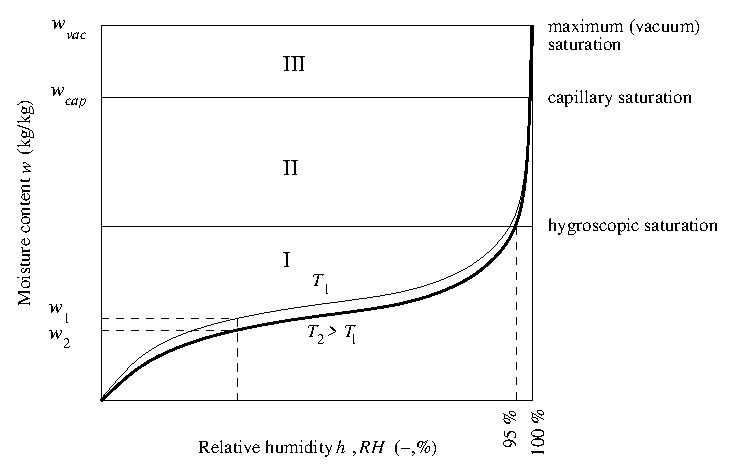
\includegraphics[angle=0, width=10cm]{PS/reten.eps}
\caption{Sorption isotherms}
\label{reten}
\end{center}
\end{figure}

In the transient region II, there is a relationship between the relative humidity, the water content (saturation) 
and the capillary pressure in the pores \cite{lewis}
\begin{eqnarray}\label{cap_press}
p^c = p^g - p^w,
\end{eqnarray}
where $p^w > 0$ is the pressure of the liquid phase (water). 

\subsubsection{Pedersen model}

\begin{center}
\begin{tabular}{|l|l|}
\hline
location & /TRFEL/SRC/bazped.cpp\\
         & /TRFEL/SRC/bazped.h\\
         & /TRFEL/SRC/pedersen.cpp\\
         & /TRFEL/SRC/pedersen.h
\\ \hline
related files &
\\ \hline
notes & 
\\ \hline
\end{tabular}
\end{center}

The sorption isotherm is approximated by this simple formula \cite{pedersen}
\begin{eqnarray}\label{sorption_isotherm}
w = w_h \Big(1 - \frac{\ln h}{A}\Big)^{-\frac{1}{n}},
\end{eqnarray}
where $h$ is relative humidity and $w_h$, $A$, $n$ are material parameters.

An analytical expression is proposed for the saturation vapor pressure as a function of temperature $T[{\rm K}]$ 
\begin{eqnarray}\label{saturation_pressure}
p^{gws}(T) = \exp \Big(23,5771 - \frac{4042,9}{T-37,58}\Big) \quad ({\rm Pa}).
\end{eqnarray}

\subsubsection{JM model}
\begin{center}
\begin{tabular}{|l|l|}
\hline
location & /TRFEL/SRC/kunzel.cpp\\
         & /TRFEL/SRC/kunzel.h
\\ \hline
related files &
\\ \hline
notes & 
\\ \hline
\end{tabular}
\end{center}


%%%%%%%%%%%%%%%%%%%%%%%%%%%%%%%%%%%%%%%%%%%%%%%%%%%%%%%%
\subsection{Models for water vapor permeability}
As for the {\it water vapor transport}, studies of experimental data of concrete have indicated that permeability 
varies tremendously with temperature especially at temperature levels close to 100$^\circ$C. 
Introducing water vapor permeabilty as a scalar variable,
\begin{eqnarray}
\delta^{gw} = \frac{k^{rgw}k_{sat}}{\nu^{gw}} \quad ({\rm s}),
\end{eqnarray}
and denoting its maximum as $\delta_{wet}^{gw}$, the two possible diagrams of the water vapor permeability displayed 
in Fig.~\ref{s_shape} as a function of relative humidity  $RH = h$ and moisture content $w$, respectively, 
are plausible approximations of this dependence.
\begin{figure}[h!]
\begin{center}
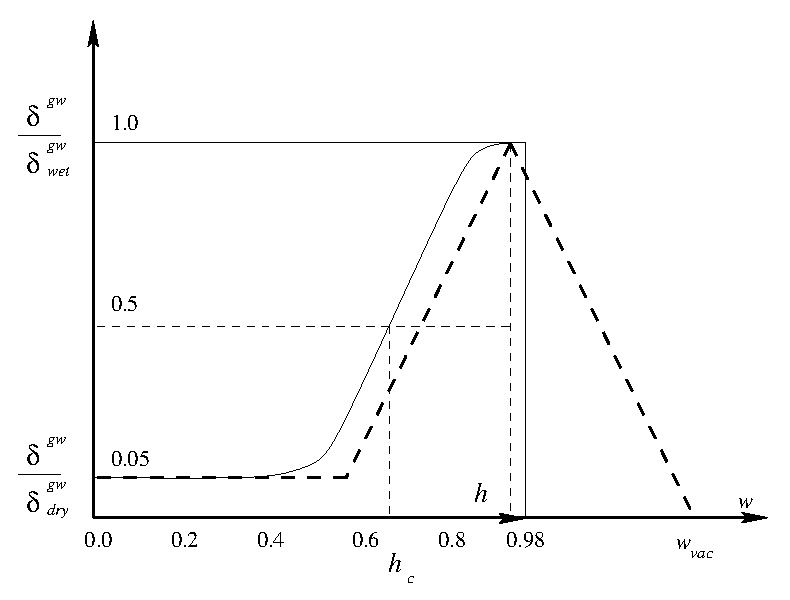
\includegraphics[angle=0, width=10cm]{PS/s_shape.eps}
\caption{Distribution of water vapor permeability as a function of $h$ and $w$}
\label{s_shape}
\end{center}
\end{figure}

\subsubsection{Bazant model}

\begin{center}
\begin{tabular}{|l|l|}
\hline
location & /TRFEL/SRC/bazped.cpp\\
         & /TRFEL/SRC/bazped.h
\\ \hline
related files &
\\ \hline
notes & 
\\ \hline
\end{tabular}
\end{center}

The solid S-shaped curve was proposed by Z. P. Ba\v{z}ant and L. J. Njjar in~\cite{bazant_n} using a function 
with three parameters $a_0$, $h_c$, $n$
\begin{equation}
\frac{\delta^{gw}}{\delta_{\rm wet}^{gw}} = a_0 + \frac{1 -a_0}{1 + \big(\frac{1 - h}{1 - h_c}\big)^n},
\end{equation}
where parameter $h_c$ characterizes the relative humidity at which $\delta^{gw}/\delta_{wet}^{gw}$ drops half-way between 
its maximum and minimum values. The dashed line was considered by \cite{pedersen}.


\subsubsection{Pedersen model}

\begin{center}
\begin{tabular}{|l|l|}
\hline
location & /TRFEL/SRC/pedersen.cpp\\
         & /TRFEL/SRC/pedersen.h
\\ \hline
related files &
\\ \hline
notes & 
\\ \hline
\end{tabular}
\end{center}

The dashed line was considered by \cite{pedersen}:
\begin{equation}
\delta^{gw} = \delta^{gw}_{\rm dry} + \frac{h-0.60}{0.98-h}(\delta^{gw}_{\rm wet} - \delta^{gw}_{\rm dry}),\nonumber
\end{equation}
if $h$ $\leq$ 0.60:
\begin{equation}
\delta^{gw} = \delta^{gw}_{\rm dry},\nonumber
\end{equation}
if $h$ $\geq$ 0.98:
\begin{equation}
\delta^{gw} = \delta^{gw}_{\rm wet}\frac{w_{\rm cap} - w}{w_{\rm vac} - w_{98}},\nonumber
\end{equation}
if $w$ $>$ $w_{\rm vac}$:
\begin{equation}
\delta^{gw} = 0.\nonumber
\end{equation}

%%%%%%%%%%%%%%%%%%%%%%%%%%%%%%%%%%%%%%%%%%%%%%%%%%%%%%%%
\subsection{Models for hydraulic conductivity}
\subsubsection{Pedersen model}

\begin{center}
\begin{tabular}{|l|l|}
\hline
location & /TRFEL/SRC/bazped.cpp\\
         & /TRFEL/SRC/bazped.h\\
         & /TRFEL/SRC/pedersen.cpp\\
         & /TRFEL/SRC/pedersen.h
\\ \hline
related files &
\\ \hline
notes & 
\\ \hline
\end{tabular}
\end{center}

For the {\it liquid transport} the following expressions are proposed in \cite{pedersen} to describe, 
in case of uniaxial flow, the dependence of the so called hydraulic conductivity, $K^w/g$ (s), 
on the moisture content $w$:
\begin{equation}\label{20}
\begin{array}{rl} 
w < w_{cr}, & K^w/g \doteq 0,\\
w_{cr} \leq w \leq w_{cap}, & K^w/g = A_k {\rm exp} \big(B_kw \big),\\
w_{cap} < w, & K^w/g = A_k {\rm exp} \big(B_kw_{cap} \big),
\end{array}
\end{equation}
where $A_k,B_k$ are coefficients yet to be determined from experiments.


%%%%%%%%%%%%%%%%%%%%%%%%%%%%%%%%%%%%%%%%%%%%%%%%%%%%%%%%
%%%%%%%%%%%%%%%%%%%%%%%%%%%%%%%%%%%%%%%%%%%%%%%%%%%%%%%%
\section{Models for coupled heat and moisture transfer}
\subsection{Mass and heat transfer in deforming porous media \\- a review of Lewis' and Schrefler's theory}
\label{keynote}
{\bf Constitutive relations}

Moisture in materials can be present as moist air, water and ice or in some intermediate state as adsorbed phase 
on the pore walls, respectively. Since it is in general not possible to distinguish the different aggregate states, 
the water content $w$ is defined as the ratio of the total moisture weight (kg/kg) to the dry weight of the material. 
\begin{eqnarray}\label{w_S}
(1-n) \rho^sw = nS_w\rho^w + nS_g\rho^g, \qquad S_w + S_g = 1,
\end{eqnarray}
The degree of saturation $S_w$ is a function of capillary pressure $p^c$ and temperature $T$, 
which is determined experimentally
\begin{equation}\label{Sw}
S_w = S_w(p^c,T).
\end{equation}
The capillary pressure $p^c$ id defined as
\begin{equation}\label{pc}
p^c = p^g - p^w,
\end{equation}
where $p^w > 0$ is the pressure of the liquid phase (water). 

The pressure of the moist air, $p^g > 0$, in the pore system is usually considered as the pressure in a perfect 
mixture of two ideal gases - dry air, $p^{ga}$, and water vapor, $p^{gw}$, i.e.,
\begin{equation}\label{ungas}
p^g = p^{ga} + p^{gw}=\Big( \frac{\rho^{ga}}{M_a} + \frac{\rho^{gw}}{M_w} \Big)T 
R = \frac{\rho^{g}}{M_g}T R.
\end{equation}
In this relation $\rho^{ga}, \rho^{gw}$ and $\rho^{g}$ stand for the respective intrinsic phase densities, $T$ 
is the absolute temperature, and $R$ is the universal gas constant.
 
Identity \eqref{ungas} defining the molar mass of the moist air, $M_g$, in terms of the molar masses of individual 
constituents is known as Dalton's law. The capillary pressure is larger the smaller the capillary radius is. It is shown 
thermodynamically that the capillary pressure can be expressed unambiguously by the relative humidity $RH$ using 
the Kelvin-Laplace law
\begin{equation}\label{kelvinlapl}
RH = \frac{p^{gw}}{p^{gws}} = {\rm exp} \Big( - \frac{p^c M_w}{\rho^w R T} \Big).
\end{equation}
The water vapor saturation pressure, $p^{gws}$, is a function of the temperature only and can be expressed by the 
Clausius-Clapeyron equation
\begin{equation}\label{clausius}
p^{gws}(T) = p^{gws}(T_0) {\rm exp} \Big[ - \frac{M_w \Delta h_{\rm vap}}{R} \Big(\frac{1}{T} - 
\frac{1}{T_0} \Big) \Big],
\end{equation}
where $T_0$ is a reference temperature and $\Delta h_{\rm vap}$ is the specific enthalpy of saturation.

Materials having heat capacities is the term deliberately used 
to emphasize the similarity to the description of the moisture retention. It is simply expressed as
\begin{equation}
H =H(T),
\end{equation}
where $H$ is the mass specific enthalpy (J.kg$^{-1}$), $T$ - temperature (K).

It is not common to write the enthalpy in an absolute way as here. Instead, changes of enthalpy are 
described in a differential way, which leads to the definition of the specific heat capacity as the slope 
of the $H - T$ curve, i.e.
\begin{equation}\label{cap}
C_p = \Big( \frac{\partial H}{\partial T}\Big)_{p={\rm const.}}.
\end{equation}
The heat capacity varies insignificantly with temperature. It is customary, however, to correct this term 
for the presence of the fluid phases and to introduce the effective heat capacity as
\begin{equation}
\big( \rho C_p \big)_{\rm eff} = \rho_s C_{ps} + \rho_w C_{pw} + \rho_g C_{pg}.
\end{equation}

{\bf Transfer equations}

The mass averaged relative velocities, $\tenss{v} ^{\alpha} - \tenss{v} ^s$, are expressed 
by the generalized form of {\bs {Darcy's law}} \cite{lewis}
\begin{equation}\label{darcy}
n S_{\alpha} \big( \tenss{v} ^{\alpha} - \tenss{v} ^s \big) = \frac{k^{r\alpha} \tenss{k}_{sat}}
{\mu^{\alpha}} \big( - {\rm grad} p^{\alpha} + \rho^{\alpha} \tenss{g} \big),
\end{equation}
where $\alpha = w$ for the liquid phase and $\alpha = g$ for the gaseous phase.

Dimensionless relative permeabilities $k^{r\alpha} \in \langle 0,1 \rangle$ are functions of degree of~
saturation
\begin{equation}
k^{r\alpha} = k^{r\alpha} (S_w)\qquad ({\rm m \cdot s}^{-1}).
\end{equation}

In Equation (\ref{darcy}), $\tenss{k}_{sat}$ (m$^2$) is the square (3x3) intrinsic permeability matrix 
 and $\mu^{\alpha}$ is the dynamic viscosity (kg.m$^{-1}$.s$^{-1}$). The intrinsic mass densities $\rho^{\alpha}$ 
are related to the volume averaged mass densities $\rho_{\alpha}$ through the relation
\begin{equation}\label{av_dens}
\rho_{\alpha} = n S_{\alpha} \rho^{\alpha}.
\end{equation}
The relative permeability $k^{rw}$ goes to zero, when water saturation $S_w$ approaches $S_{irr}$, 
which is the limiting value of $S_w$ as the suction stress approaches infinity (\cite{fatt}).

Diffusive-dispersive mass flux (kg.m$^{-2}$.s$^{-1}$) of the water vapor ($gw$) in the gas
 ($g$) is the second driving mechanism. It is governed by {\bs {Fick's law}}
\begin{equation}\label{fick}
\tenss{J}^{gw}_g = n S_g \rho^{gw} \big( \tenss{v} ^{gw} - \tenss{v} ^g \big) = - \rho^g \tenss{D}^{gw}_g 
{\rm grad} \Big( \frac{\rho^{gw}}{\rho^g} \Big),
\end{equation}
where $\tenss{D}^{gw}_g$ (m$^2$.s$^{-1}$) is the effective dispersion tensor. It can be shown \\ \cite{lewis} that
\begin{equation}
\tenss{J}^{gw}_g = - \rho^g \frac{M_a M_w}{M^2_g} \tenss{D}^{gw}_g {\rm grad} \Big( \frac{\rho^{gw}}{\rho^g} \Big)
= \rho^g \frac{M_a M_w}{M^2_g} \tenss{D}^{ga}_g {\rm grad} \Big( \frac{\rho^{ga}}{\rho^g} \Big) = - \tenss{J}^{ga}_g.
\end{equation}
Recall that $\tenss{D}^{gw}_g = \tenss{D}^{ga}_g = \tenss{D}_g$.
Here, $\tenss{J}_g^{ga}$ is the diffusive-dispersive mass flux of the dry air in the gas.

Conduction of heat in normal sense comprises radiation as well as convective heat transfer on a 
microscopic level. The generalized version of {\bs {Fourier's law}} is used to describe the conduction
 heat transfer
\begin{equation}\label{fourier}
\tenss{q} = - \tenss{\chi}_{\rm eff} {\rm grad} T,
\end{equation}
where $\tenss{q}$ is the heat flux (W.m$^{-2}$), $\tenss{\chi}_{\rm eff}$ is the effective thermal conductivity matrix 
(W.m$^{-1}$.K$^{-1}$).

The thermal conductivity increases with increasing temperature due to the non-linear 
behavior of the microscopic radiation, which depends on difference of temperatures raised to the 
$4^{\rm{th}}$ power. Presence of water also increases the thermal conductivity. A suitable formula
reflecting this effect can be found in \cite{lewis}.

{\bf Deformation of solid skeleton. Concept of effective stress}

The stresses in the grains, $\tenss{\sigma}^s$, can be expressed using a standard averaging technique 
in terms of the stresses in the liquid phase, $\tenss{\sigma}^w$, the stresses in the gas, $\tenss{\sigma}^g$, 
and the effective stresses between the grains, $\tenss{\sigma}^{ef}$. The equivalence conditions for the internal 
stresses and for the total stress $\tenss{\sigma}$ lead to the expression~\cite{bitt}.
\begin{equation}\label{d3}
\tenss{\sigma} = \tenss{\sigma}^{ef} + S_w \tenss{\sigma}^w + S_g \tenss{\sigma}^g + \Delta \tenss{\tau}.
\end{equation}
Assuming that the shear stress $\tenss{\tau}$ in fluids is negligible converts the latter equation into the form
\begin{equation}\label{d4}
\tenss{\sigma} = \tenss{\sigma}^{ef} - p^s \tenss{m},
\end{equation}
where
\begin{equation}\label{d5}
\tenss{\sigma} = \big\{ \sigma_x,\sigma_y,\sigma_z,\tau_{yz},\tau_{zx},\tau_{xy}\big\}^{\rm T}, \quad
\tenss{m} = \big\{ 1,1,1,0,0,0 \big\}^{\rm T},
\end{equation}
and
\begin{equation}\label{d6}
p^s = S_w p^w + S_g p^g.
\end{equation}

Deformation of a porous skeleton associated with the grain rearrangement can be expressed using 
the constitutive equation written in the rate form
\begin{equation}\label{d7}
\dot{\tenss{\sigma}}^{ef} = \tenss{D}_{sk} \big(\dot{\tenss{\varepsilon}} - \dot{\tenss{\varepsilon}}_0 \big).
\end{equation}
The dots denote differentiation with respect to time, $\tenss{D}_{sk} = \tenss{D}_{sk}(\dot{\tenss{\varepsilon}}, 
{\tenss{\sigma}}^{ef}, T) $ is the tangential matrix of the porous skeleton and $\dot{\tenss{\varepsilon}}_0$ 
represents the strains that are not directly associated with stress changes (e.g., temperature effects, shrinkage, 
swelling, creep). It also comprises the strains of the bulk material due to changes of the pore pressure
\begin{equation}\label{d8}
\dot{\tenss{\varepsilon}} =  -\tenss{m} \Big( \frac{\dot{p}^s}{3K_s} \Big),
\end{equation}
where $K_s$ is the bulk modulus of the solid material (matrix).

When admitting only this effect and combining Equations (\ref{d4}), (\ref{d7}) and (\ref{d8}), we get
\begin{equation}\label{d9}
\dot{\tenss{\sigma}} = \dot{\tenss{\sigma}}^{ef} - \dot{p}^s \tenss{m} = \tenss{D}_{sk} \dot{\tenss{\varepsilon}}
- \alpha \tenss{m} \dot{p}^s = \dot{\tenss{\sigma}}'' - \alpha \tenss{m} \dot{p}^s,
\end{equation}
where
\begin{equation}\label{d10}
\alpha = \frac{1}{3} \tenss{m}^{\rm T} \Big( \tenss{I} - \frac{\tenss{D}_{sk}}{3K_m} \Big) \tenss{m} = 1 - 
\frac{K_{sk}}{K_s} < 1,
\end{equation}
and $K_{sk} = \tenss{m}^{\rm T} \tenss{D}_{sk} \tenss{m}/9$ is the bulk modulus of the porous skeleton. 
For a material without any pores, $K_{sk} = K_s$. For cohesive soils, $K_{sk} << K_s$ and $\alpha = 1$. 
The above formulas are also applicable to long-term deformation of rocks, for which  $\alpha \leq 0.5$, 
and this fact strongly affects Equation (\ref{d9}) \cite{zienkiewicz83}.

Changes of the effective stress along with temperature and pore pressure changes produce change of the solid density 
$\dot{\rho}^s$. To derive the respective material relation for this quantity, we start from the mass conservation equation 
for the solid phase. In the second step we introduce the constitutive relationship for the mean effective stress expressed 
in terms of quantities describing the deformation of the porous skeleton. After some manipulations we arrive at the 
searched formula
\begin{equation}\label{d15}
(1 - n)\frac {\dot{\rho}^s}{\rho^s} = (\alpha - n)\Big(\frac {\dot{p}^s}{K_s} - \beta_s \dot{T}\Big) + 
(\alpha - 1){\rm div} \tenss{v}^s,
\end{equation}
where $\beta_s$ is the thermal expansion coefficient of the solid phase.

Similar approach applied to the mass conservation equation of the liquid phase leads to the following constitutive equation
\begin{equation}\label{d16}
\frac {\dot{\rho}^w}{\rho^w} = \frac {\dot{p}^w}{K_w} - \beta_s \dot{T},
\end{equation}
where $K_w$ is the bulk modulus of water and $\beta_w$ is the thermal expansion coefficient of this phase.

{\bf Set of governing equations}

The complete set of equations describing the coupled moisture and heat transport in deforming porous media comprises 
the linear balance (equilibrium) equation formulated for a multi-phase body, the energy balance equation and 
the continuity equations for the liquid water and gas.

{\it Continuity equation for the dry air}
\begin{eqnarray}\label{air}
\frac{\partial}{\partial t}\Big(\varphi(1-S_w)\rho^{ga}\Big) + \alpha(1-S_w)\rho^{ga} {\rm div} \tenss{\dot{u}} - 
{\rm div} \Big( \rho^{ga}\frac{k^{rg}\tenss{k}_{sat}}{{\mu}^{g}} {\rm grad}p^g\Big) + \nonumber\\
+{\rm div} \Big( \rho^g \frac{M_a M_w}{M^2_g} \tenss{D}_{\rm eff} {\rm grad} \Big( \frac{p^{gw}}{p^g} \Big) \Big) = 0,
\end{eqnarray}
where $\tenss{\dot{u}}$ ($\tenss{\dot{u}} = \tenss{v}^s$) is the velocity of solid.

{ \it Continuity equation for the water species}
\begin{eqnarray}\label{water}
\frac{\partial}{\partial t}\Big(\varphi(1-S_w)\rho^{gw}\Big) + \alpha(1-S_w)\rho^{gw} {\rm div} \tenss{\dot{u}} - 
{\rm div} \Big( \rho^{gw}\frac{k^{rg}\tenss{k}_{sat}}{{\mu}^{g}} {\rm grad}p^g\Big) + \nonumber\\
-{\rm div} \Big( \rho^g \frac{M_a M_w}{M^2_g} \tenss{D}_{\rm eff} {\rm grad} \Big( \frac{p^{gw}}{p^g} \Big) \Big) = \nonumber\\
=-\frac{\partial}{\partial t}\Big(\varphi S_w\rho^{w}\Big) - \alpha S_w \rho^{w} {\rm div} \tenss{\dot{u}} + 
{\rm div} \Big( \rho^{w}\frac{k^{rw}\tenss{k}_{sat}}{{\mu}^{w}} ({\rm grad}p^g - {\rm grad}p^c - \rho^w\tenss{g})\Big)
\end{eqnarray}

{ \it Energy balance equation}
 \begin{eqnarray}\label{heat}
\big( \rho C_p \big)_{\rm eff} \frac{\partial T}{\partial t} - {\rm div}\big(\lambda_{\rm eff}{\rm grad}T\big) + \nonumber\\
- \Big(C_{pw} \rho^w \frac{k^{rw}\tenss{k}_{sat}}{{\mu}^{w}} ({\rm grad}p^g - {\rm grad}p^c - \rho^w\tenss{g}) + 
C_{pg} \rho^{gw}  \frac{k^{rg}\tenss{k}_{sat}}{{\mu}^{g}} {\rm grad}p^g\Big) {\rm grad}T = \nonumber\\
=\Delta h_{\rm vap} \Big[\frac{\partial}{\partial t}\Big(\varphi S_w\rho^{w}\Big) + \alpha S_w \rho^{w} {\rm div} \tenss{\dot{u}} -
{\rm div} \Big( \rho^{w}\frac{k^{rw}\tenss{k}_{sat}}{{\mu}^{w}} ({\rm grad}p^g - {\rm grad}p^c - \rho^w\tenss{g})\Big)\Big]
\end{eqnarray}

The { \it equilibrium equation} (the linear balance equation) must yet be introduced to complete a set of governing 
equations
\begin{equation}\label{d19}
{\rm div} \big(\tenss{\sigma} - \tenss{m}(p^g - S_w p^c)\big)+ \rho \tenss{g} = \tenss{\rm 0}
\end{equation}
with density of the multi-phase medium defined as
\begin{equation}\label{d20}
\rho = (1-n)\rho^s + nS_w\rho^w + nS_g\rho^g = \rho_s + \rho_w + \rho_g.
\end{equation}

{ \it Initial and boundary conditions}

The initial conditions specify the full fields of gas pressure, capillary or water pressure, 
temperature and displacement and velocities:
\begin{equation}\label{init}
p^g = p^g_0, \qquad p^c = p^c_0, \qquad T = T_0, \qquad \tenss{u} = \tenss{u}_0, 
\quad {\rm and}  \quad \dot{\tenss{u}} = \dot{\tenss{u}}_0, \quad {\rm at}\quad t = 0. 
\end{equation}
The boundary conditions can be imposed values on $\Gamma^1_{\pi}$ or fluxes on $\Gamma^2_{\pi}$, where the boundary
$\Gamma = \Gamma^1_{\pi} + \Gamma^2_{\pi}$.
\begin{equation}\label{bound1}
p^g = \overline{p}^g \quad {\rm on} \quad \Gamma^1_{g}, \quad p^c = \overline{p}^c \quad {\rm on} \quad \Gamma^1_{c},
\quad T = \overline{T} \quad {\rm on} \quad \Gamma^1_{T}, \quad \tenss{u} = \overline{\tenss{u}}  \quad {\rm on} \quad \Gamma^1_{u}.
\end{equation}
The volume averaged flux boundary conditions for water species and dry air conservation equations 
and energy equation to be imposed at the interface between the porous medium and the surrounding fluid are as follows
\begin{eqnarray}\label{bound2}
\big(\rho^{ga}\tenss{J}^{ga} - \rho^{g}\tenss{J}^{gw}\big)\cdot\tenss{n} &=& q_{ga} \quad {\rm on} \quad \Gamma^2_{g}\nonumber\\
\big(\rho^{gw}\tenss{J}^{ga} + \rho^{w}\tenss{J}^{w} + \rho^{g}\tenss{J}^{gw}\big)\cdot\tenss{n} &=& 
\beta_c(\rho^{gw} -\rho^{gw}_{\infty}) + q_{gw} + q_{w}\quad {\rm on} \quad \Gamma^2_{c}\\
-\big(\rho^{w}\tenss{J}^{w}\Delta h_{\rm vap} - \lambda_{\rm eff}{\rm grad}T)\cdot\tenss{n} &=& 
\alpha_c(T - T_{\infty}) + q_{T}\quad {\rm on} \quad \Gamma^2_{T}\nonumber
\end{eqnarray}
where $\tenss{n}$ is the unit normal vector of the surface of the porous medium, $\rho^{gw}_{\infty}$ and $T_{\infty}$ 
are the mass concentration of water vapor and temperature in the undisturbed gas phase far away from the interface, 
and $q_{ga}$, $q_{gw}$, $q_w$ and $q_T$ are the imposed air flux, the imposed vapor flux, the imposed liquid flux and 
the imposed heat flux, respectively.

The traction boundary conditions for displacement field are:
\begin{equation}\label{bound3}
\sigma\cdot\tenss{n} = \tenss{t} \quad {\rm on} \quad \Gamma^2_{u}
\end{equation}
where $\tenss{t}$ is the imposed traction.

\subsubsection{Discretization of governing equations}

A weak formulation of the governing equations \eqref{air} to \eqref{d19} is obtained by applying Galerkin's method
of weighted residuals. For the numerical solution, the governing equations are discretized in space by means of the 
finite element method, yielding a non-symmetric and non-linear system of partial differential equations:
\begin{eqnarray}\label{final1}
\tenss{K}_{uu}\tenss{u} + \tenss{K}_{ug}\tenss{p}_g + \tenss{K}_{uc}\tenss{p}_c + \tenss{K}_{ut}\tenss{T} &=& \tenss{F}_u,\nonumber\\
\tenss{C}_{gg}\tenss{\dot{p}}_g + \tenss{C}_{gc}\tenss{\dot{p}}_c + \tenss{C}_{gt}\tenss{\dot{T}} +\tenss{C}_{gu}\tenss{\dot{u}} + 
\tenss{K}_{gg}\tenss{p}_g + \tenss{K}_{gc}\tenss{p}_c + \tenss{K}_{gt}\tenss{T} &=& \tenss{F}_g,\nonumber\\
\tenss{C}_{cg}\tenss{\dot{p}}_g + \tenss{C}_{cc}\tenss{\dot{p}}_c + \tenss{C}_{ct}\tenss{\dot{T}} + \tenss{C}_{cu}\tenss{\dot{u}} + 
\tenss{K}_{cg}\tenss{p}_g + \tenss{K}_{cc}\tenss{p}_c + \tenss{K}_{ct}\tenss{T} &=& \tenss{F}_c,\\
\tenss{C}_{tg}\tenss{\dot{p}}_g + \tenss{C}_{tc}\tenss{\dot{p}}_c + \tenss{C}_{tt}\tenss{\dot{T}} + \tenss{C}_{tu}\tenss{\dot{u}} + 
\tenss{K}_{tg}\tenss{p}_g + \tenss{K}_{tc}\tenss{p}_c + \tenss{K}_{tt}\tenss{T} &=& \tenss{F}_t.\nonumber
\end{eqnarray}
The equations \eqref{final1} can be rewritten in concise form as
\begin{equation}\label{final2}
\tenss{K}(\tenss{X})\tenss{X} + \tenss{C}(\tenss{X})\tenss{\dot{X}} = \tenss{F}(\tenss{X}),
\end{equation}
where $\tenss{X}^{\rm T} = \{\tenss{p}^g,\tenss{p}^c,\tenss{T},\tenss{u}\}$, $\tenss{C}(\tenss{X})$ is ``the general capacity matrix'', 
$\tenss{K}(\tenss{X})$ is ``the general conductivity matrix'' and are obtained together with $\tenss{F}(\tenss{X})$ 
by assembling the sub-matrices indicated in equations \eqref{final1}. The dot denotes the time derivative.


The matrices appearing in Equation \eqref{final1} are shown here in detail in~\cite{pesavento}\\
(\textsf {http://cml.fsv.cvut.cz/\~{}sifel}), using the notation of Lewis and Schrefler~\cite{lewis}.
%\begin{eqnarray}
%\tenss{K}_{uu} &=&\\
%\tenss{K}_{ug} &=&\\
%\tenss{K}_{uc} &=&\\
%\tenss{K}_{ut} &=&\\
%\tenss{F}_u &=&\\
%\tenss{C}_{gg} &=&\\
%\tenss{C}_{gc} &=&\\
%\tenss{C}_{gt} &=&\\
%\tenss{C}_{gu} &=&\\ 
%\tenss{K}_{gg} &=&\\
%\tenss{K}_{gc} &=&\\
%\tenss{K}_{gt} &=&\\
%\tenss{F}_g &=&\\
%\tenss{C}_{cg} &=&\\
%\tenss{C}_{cc} &=&\\
%\tenss{C}_{ct} &=&\\
%\tenss{C}_{cu} &=&\\ 
%\tenss{K}_{cg} &=&\\
%\tenss{K}_{cc} &=&\\
%\tenss{K}_{ct} &=&\\
%\tenss{F}_c &=&\\
%\tenss{C}_{tg} &=&\\
%\tenss{C}_{tc} &=&\\
%\tenss{C}_{tt} &=&\\
%\tenss{C}_{tu} &=&\\ 
%\tenss{K}_{tg} &=&\\
%\tenss{K}_{tc} &=&\\
%\tenss{K}_{tt} &=&\\
%\tenss{F}_t &=&
%\end{eqnarray}

\subsection{Mass and heat transfer in deforming porous media \\- a review of Glasgow theory (based on Tenchev's approach)}
\label{glasgow}
The paper containing a review of Glasgow approach is available on \textsf {http://cml.fsv.cvut.cz/\~{}sifel} 
(click on REFERENCES).

%%%%%%%%%%%%%%%%%%%%%%%%%%%%%%%%%%%%%%%%%%%%%%%%%%%%%%%%
\subsection{Coupled heat and moisture transfer in non-deforming porous medium - simplified solution (two unknowns)}
\subsubsection{Lewis' and Schrefler's approach - theory of multi-phase porous medium\\
- unknowns = $w$ [kg/kg] moisture content, $T$ [K] temperature}

{\bf Liquid and gas transport}\\

If moisture convection is neglected, the liquid and gas (moist air) transport and 
the vapor diffusion taking place in the gas are the remaining driving mechanisms.
The transport of the vapor phase is governed by Fick's law (\ref{fick})
\begin{eqnarray}\label{fick_2}
\tenss{J}^{gw}_s &=& n(1-S_w) \rho^{gw} \big( \tenss{v} ^{gw} - \tenss{v}^s \big) = 
- \frac{k^{gw}}{\nu^{gw}} {\rm grad} p^{gw}\nonumber\\
&=&-\delta^{gw}(S) {\rm grad} p^{gw}\nonumber\\
&=&-\delta^{gw}(S)\Big[\frac{\partial p^{gw}}{\partial T} {\rm grad} T + \frac{\partial p^{gw}}{\partial S} {\rm grad} 
S \Big].
\end{eqnarray}
The flux of the liquid phase (Darcy's law (\ref{darcy})) is expressed as
\begin{eqnarray}\label{darcy_2}
\tenss{J}_s^{w} &=& n S_w \rho^w \big( \tenss{v} ^{w} - \tenss{v}^s \big) = - \frac{K^w(s)}{g} {\rm grad} p^w\nonumber\\
&=& - \frac{K^w(S)}{g} {\rm grad} (p^{gw} - p^c)\nonumber\\
&=& - \frac{K^w(S)}{g}\Big[\Big(
\frac{\partial p^{gw}}{\partial T} - \frac{\partial p^{c}}{\partial T}\Big) {\rm grad} T
+ \Big(\frac{\partial p^{gw}}{\partial S} - \frac{\partial p^{c}}{\partial S}\Big) {\rm grad} S \Big].
\end{eqnarray}
It remains to calculate the partial derivatives of $p^{gw}$ and $p^c$ with respect to $T$ and $S$.

As $p^{gw} = h p^{gws}$ we have
\begin{eqnarray}
\frac{\partial p^{gw}}{\partial T} = \frac{\partial}{\partial T} \Big(h p^{gws}(T)\Big)\Big|_{h = {\rm const}} 
= h \frac{\partial p^{gws}(T)}{\partial T}.
\end{eqnarray}
Making use of the Kelvin-Laplace law (\ref{kelvinlapl}) yields
\begin{eqnarray}
\frac{\partial p^{c}}{\partial T} = \frac{\partial}{\partial T} \Big[-\frac{\rho^w R T}{M_w}\ln h \Big]_{h = {\rm const}} 
= -\frac{\rho^w R}{M_w}\ln h.
\end{eqnarray}
If $h$ approaches one, $S > S_{\rm irr}$ (II. and III. region) then 
\begin{eqnarray}\label{region}
\frac{\partial p^{gw}}{\partial T} \rightarrow \frac{{\rm d} p^{gws}(T)}{{\rm d} T} 
\qquad {\rm and} \quad \frac{\partial p^{c}}{\partial T}\rightarrow 0.
\end{eqnarray}
\begin{eqnarray}
\frac{{\rm d} w(S)}{{\rm d} S}  &=& \frac{n(\rho^w - \rho^g)}{(1-n)\rho^s} 
\approx \frac{n}{1-n}\frac{(\rho^w - \rho^{gw})}{\rho^s} \doteq {\rm const}.
\end{eqnarray}
Proceeding in a standard way, we find the partial derivative
\begin{eqnarray}
\frac{\partial p^{gw}}{\partial S}\Big|_{T = {\rm const}} &=& 
\frac{\partial p^{gw}}{\partial h} \cdot \frac{\partial h}{\partial w}
\cdot \frac{\partial w}{\partial S}\nonumber\\
&=& \frac{\partial p^{gw}}{\partial w} \frac{n}{1-n}\frac{(\rho^w - \rho^{gw})}{\rho^s}
\end{eqnarray}
where
\begin{eqnarray}
\frac{\partial p^{gw}}{\partial w} = p^{gws}(T) \frac{{\rm d} h(w)}{{\rm d} w}.
\end{eqnarray}
There are two possibilities how to evaluate the partial derivative of $p^c$ with respect to $\varPsi = S, w, h$:
\begin{itemize}
\item{by starting from formula (\ref{Sw}) to get}
\begin{eqnarray}
\frac{\partial p^{c}}{\partial \varPsi} = \frac{\partial p^{c}(S)}{\partial S} \cdot \frac{\partial S}{\partial \varPsi}
\end{eqnarray}
\item{or by exploiting the Kelvin - Laplace equation (\ref{kelvinlapl})}
\end{itemize}
\begin{eqnarray}
\frac{\partial p^{c}}{\partial \varPsi} = \frac{\partial p^{c}}{\partial h}\Big|_{T = {\rm const}} 
\cdot \frac{\partial h}{\partial \varPsi},
\quad {\rm where} \quad \frac{\partial p^{c}}{\partial h}\Big|_{T = {\rm const}} = -\frac{\rho^w R T}{M_w} 
\frac{{\rm d}(\ln h)}{{\rm d} h} = 
- \frac{\rho^w R T}{M_w} \frac{1}{h}
\end{eqnarray}

{\bf Mass balance equation for two-phase zone}\\

The mass balance equation for the liquid phase reads 
\begin{eqnarray}\label{masswater}
\frac{\partial \big( n S_w \rho^w\big)}{\partial t} + {\rm div} \big[n S_w \rho^w \tenss{v}^w\big]
 = -\dot{m}.
\end{eqnarray}
The effect of dry air can be neglected in the transition region for $S > S_{\rm irr}$ (two-phase zone). 
Then $S_{gw} \doteq 1-S_{w} = 1-S$ and the mass balance equation for vapor assumes this form
\begin{eqnarray}\label{massvapor_2}
\frac{\partial \big[n(1- S_w) \rho^{gw}\big]}{\partial t} + {\rm div} \big[n (1-S_w)
\rho^{gw} \tenss{v}^{gw}\big] = \dot{m}.
\end{eqnarray}
By adding Eqs. (\ref{masswater}) and (\ref{massvapor_2}) considering Eq. (\ref{w_S}) and substituting from 
Eqs. (\ref{fick_2}) and (\ref{darcy_2}), 
we arrive at the mass balance equation in two-phase zone of a porous material:
\begin{eqnarray}\label{twophase}
\rho_s \frac{\partial w}{\partial t} = \frac{\partial w(\varPsi)}{\partial \varPsi} 
\cdot \frac{\partial \varPsi}{\partial t} = 
{\rm div} \big( a_{\varPsi T}(\varPsi, T) {\rm grad} T + a_{\varPsi \varPsi}(\varPsi, T){\rm grad} \varPsi \big),
\end{eqnarray}
where $\rho_s = (1 - n)\rho^s$ (see Eq.~\eqref{av_dens}), $\varPsi = S, w, h$, and
\begin{eqnarray}\label{a_phi}
a_{\varPsi T}(\varPsi, T) &=& \Big[\Big( \delta^{gw}(\varPsi) + \frac{K^w(\varPsi)}{g} \Big) 
\frac{\partial p^{gw}}{\partial T} - \frac{K^w(\varPsi)}{g} \frac{\partial p^{c}}{\partial T} \Big]_{\varPsi = 
{\rm const}}\nonumber\\
a_{\varPsi \varPsi}(\varPsi, T) &=& \Big[\Big( \delta^{gw}(\varPsi) + \frac{K^w(\varPsi)}{g} \Big) 
\frac{\partial p^{gw}}{\partial \varPsi} - \frac{K^w(\varPsi)}{g} \frac{\partial p^{c}}{\partial \varPsi} \Big]_{T = 
{\rm const}}\quad .
\end{eqnarray}
If water vapor diffusion is the only driving mechanism, the preceding equations (\ref{a_phi}) simplify as
\begin{eqnarray}
a_{\varPsi T}(\varPsi, T) &=& \delta^{gw}(\varPsi) \frac{\partial p^{gw}}{\partial T}\Big|_{\varPsi = 
{\rm const}}\nonumber\\
a_{\varPsi \varPsi}(\varPsi, T) &=& \delta^{gw}(\varPsi) \frac{\partial p^{gw}}{\partial \varPsi} \Big|_{T = 
{\rm const}}\quad .
\end{eqnarray}
In the two-phase zone $S$ is always greater than $S_{\rm irr}$ (i.e. $h > 0.9$) and, in addition to Eqs. (\ref{region}), 
$\partial p^{gw}/\partial S \rightarrow 0$.\\

{\bf Energy balance equation}\\

The complete set of equations describing the coupled moisture and heat transport in porous media comprises 
the energy balance equation and the continuity equations for the liquid water and gas. 
The {\it energy balance equation} has already been derived in Paragraph~\ref{keynote} (Eq. (\ref{heat})).

The effect of evaporation (latent heat) is represented by the last term appearing on the right-hand 
side of Eq. (\ref{heat}). Neglecting convective terms and assuming rigid porous matrix yields 
the resulting form of the equation of energy conservation:
\begin{eqnarray}\label{enrg_con_first}
( \rho C)_{\rm eff} \frac{\partial T}{\partial t} &=& {\rm div} \Big\{ \Big(\chi_{\rm eff} (S, 
T) + \Delta h_{\rm vap} \delta^{gw}(S) \frac{\partial p^{gw}}{\partial T} \Big) {\rm grad} T +\\ 
& &\qquad \quad + \Delta h_{\rm vap} \delta^{gw}(S) \frac{\partial p^{gw}}{\partial S} {\rm grad} S \Big\} 
- \frac{\partial}{\partial t}
\Big[\Delta h_{\rm vap} n(1-S) \rho^{gw} \Big].\nonumber
\end{eqnarray}
Since $h = \rho^{gw}/\rho^{gws}$, the source term takes this form
\begin{eqnarray}
\frac{\partial}{\partial t} \Big[\Delta h_{\rm vap} n(1-S) \rho^{gw} \Big] &=& \Delta h_{\rm vap} n h \rho^{gws} 
\frac{\partial S}{\partial t} + \Delta h_{\rm vap} n (1 - S)\rho^{gws} \frac{\partial h}{\partial t}\\
&=& \Delta h_{\rm vap} n \rho^{gws} \Big(h + (1-S)\frac{\partial h}{\partial w} \frac{\partial w}{\partial S} \Big) 
\frac{\partial S}{\partial t} = \Delta h_{\rm vap} b(S) \frac{\partial S}{\partial t}\nonumber.
\end{eqnarray}
When dealing with the coupled moisture and heat transfer, three quantities can be used to describe the moisture field. 
Denote them by $\varPsi$; 
$\varPsi = S, w, h$. 
Eq. (\ref{enrg_con_first}) can be then rewritten into this contracted form
\begin{eqnarray}
( \rho C)_{\rm eff} \frac{\partial T}{\partial t} = {\rm div} \big\{ a_{T T} (T, \Psi) {\rm grad} T + 
a_{T \Psi} (T, \Psi) {\rm grad} \Psi \big\} - \Delta h_{\rm vap} b(\Psi)\frac{\partial \Psi}{\partial t},
\end{eqnarray}
\begin{eqnarray}
a_{T T} (T, \Psi) &=& \chi_{\rm eff} (\Psi,T) + \Delta h_{\rm vap} \delta^{gw}(\Psi) \frac{\partial p^{gw}}{\partial T},
\nonumber\\
a_{T S} (T, \Psi) &=& \Delta h_{\rm vap} \delta^{gw}(\Psi) \frac{\partial p^{gw}}{\partial \Psi}.\nonumber
\end{eqnarray}

{\bf FEM formulation for coupled moisture and heat transfer}\\

The balance equation for moisture transfer $(\Psi = w(\tenss{x},t))$ reads.
\begin{eqnarray}\label{couple}
\rho_s \frac{\partial w}{\partial t} &=& - {\rm div} \big(\tenss{J}_s^{gw}+ \tenss{J}_s^w\big) \nonumber\\
&=& {\rm div} \Big\{ \delta^{gw}(w) \Big[ \frac{\partial p^{gw}}{\partial T} {\rm grad} T 
+ \frac{\partial p^{gw}}{\partial w} {\rm grad} w \Big] + \nonumber\\ &+& \frac{K^w(w)}{g} \Big[\Big(
\frac{\partial p^{gw}}{\partial T} - \frac{\partial p^{c}}{\partial T}\Big) {\rm grad} T
+ \Big(\frac{\partial p^{gw}}{\partial w} - \frac{\partial p^{c}}{\partial w}\Big) {\rm grad} w \Big]\Big\}.
\end{eqnarray}
The fluid is transferred across interfaces with the surrounding environment by means of convection 
fluxes, $\tenss{\nu}^T\tenss{J}_c^{\alpha} \dots$ $\alpha = w, gw$. This phenomenon can be expressed 
by the boundary conditions pertaining to Eq. (\ref{couple}):
\begin{itemize}
\item{either given values (an essential condition)}
\begin{eqnarray}
w=\overline{w} \qquad {\rm on} \quad \Gamma_w = \Gamma_{1w}
\end{eqnarray}
\item{or imposed fluxes (natural boundary conditions)}
\begin{eqnarray}
\tenss{\nu}^T \tenss{J}_c^{gw} = - \tenss{\nu}^T {\delta}^{gw}(w) \Big[ \frac{\partial 
p^{gw}}{\partial T} {\rm grad} T + \frac{\partial p^{gw}}{\partial w} {\rm grad} w \Big]
= \overline{q}^{gw} \quad \Gamma^{gw}
\end{eqnarray}
\end{itemize}
and
\begin{eqnarray}
\tenss{\nu}^T \tenss{J}_c^{w} = - \tenss{\nu}^T \frac{K^w(w)}{g} \Big[\Big(
\frac{\partial p^{gw}}{\partial T} - \frac{\partial p^{c}}{\partial T}\Big) {\rm grad} T
+ \Big(\frac{\partial p^{gw}}{\partial w} - \frac{\partial p^{c}}{\partial w}\Big) {\rm grad} w \Big]
= \overline{q}^{w} \quad {\rm on} \quad \Gamma^{w}\nonumber.
\end{eqnarray}
\begin{eqnarray}
{\Gamma^{gw} \cup \Gamma^w = \Gamma_{2w}}\nonumber
\end{eqnarray}	
The water vapor flux prescribed in the direction of the outward normal $\tenss{\nu}$ 
on $\Gamma^{gw}$ 
is obtained from the following formula \cite{ctu}
\begin{eqnarray}
\overline{q}^{gw} = \beta^{gw} (p_{\rm surf}^{gw} - p_{\rm air}).
\end{eqnarray}

The equation of energy conservation is of the form
\begin{eqnarray}\label{enrg_con}
( \rho C)_{\rm eff} \frac{\partial T}{\partial t} &=& {\rm div} \Big\{ \Big(\chi_{\rm eff} (w, 
T) +  \Delta h_{\rm vap} \delta^{gw}(w) \frac{\partial p^{gw}}{\partial T} \Big) {\rm grad} T +\\
&& \qquad  +\Delta h_{\rm vap} \delta^{gw}(w) \frac{\partial p^{gw}}{\partial w} {\rm grad} w \Big\} +  \Delta h_{\rm vap} b(w) 
\frac{\partial}{\partial t}\nonumber
\end{eqnarray}
where
\begin{eqnarray}
 \Delta h_{\rm vap} b(w) =  \Delta h_{\rm vap} n \rho^{gws} \Big( h(w) + (1-S)\frac{{\rm d} h}{{\rm d} w}\Big )
\overline{q}^{gw} = \beta^{gw} (p_{\rm surf}^{gw} - p_{\rm air}).
\end{eqnarray}
The boundary conditions belonging to Eq. (\ref{enrg_con}) are
\begin{itemize}
\item{either the given values}
\begin{eqnarray}
T = \overline{T} \qquad {\rm on} \quad \Gamma_{T} = \Gamma_{1 T}
\end{eqnarray}
\item{or imposed flux. It is given as the sum of three individual fluxes - a convection exchange 
of heat between outer surfaces and the air, the absorption of a fraction of the sun radiation 
heat, and the loss of heat due to latent heat of moisture vaporization. The result reads}
\end{itemize}
\begin{eqnarray}
\tenss{\nu}^T q = - \tenss{\nu}^T \chi_{\rm eff}(w,T) {\rm grad} T  = 
\big(\beta_c + \beta_r(T)\big) \big(T_{\rm surf} - T_{\rm air}\big) + \beta_c \tenss{\nu}^T 
\tenss{J}_c^{gw}= \overline{q}_{T}\nonumber\\
{\rm on} \quad \Gamma^{T} = \Gamma_{2 T}.
\end{eqnarray}

{\bf Numerical solution}\\

Applying Galerkin's method (see Paragraph~\ref{secnonstationary}) we obtain a system of equations 
for coupled moisture and heat transfer:
\begin{eqnarray}\label{final_eq}
\left[ \begin{array}{cc}
\tenss{K}_{ww} & \tenss{K}_{wT} \\
\tenss{K}_{Tw} & \tenss{K}_{TT}
\end{array} \right]
\left\{ \begin{array}{c}
\tenss{r}_w \\
\tenss{r}_{T}
\end{array} \right\} + 
\left[ \begin{array}{cc}
\tenss{C}_{ww} & \tenss{C}_{wT} \\
\tenss{C}_{Tw} & \tenss{C}_{TT}
\end{array} \right]
\left\{ \begin{array}{c}
\dot{\tenss{r}}_w \\
\dot{\tenss{r}}_{T}
\end{array} \right\} = 
\left\{ \begin{array}{c}
\tenss{q}_{w} + \tenss{q}_{gw} \\
\tenss{q}_{T}
\end{array} \right\},
\end{eqnarray}

where
\begin{eqnarray}
\tenss{K}_{ww} = \int_{\Omega} \tenss{B}^T k_{ww} \tenss{B}{\rm d}\Omega,
\qquad \tenss{K}_{wT} = \int_{\Omega} \tenss{B}^T k_{wT} \tenss{B}{\rm d}\Omega,
\end{eqnarray}
\begin{eqnarray}
\tenss{K}_{Tw} = \int_{\Omega} \tenss{B}^T k_{Tw} \tenss{B}{\rm d}\Omega,
\qquad \tenss{K}_{TT} = \int_{\Omega} \tenss{B}^T k_{TT} \tenss{B}{\rm d}\Omega,
\end{eqnarray}
\begin{eqnarray}
\tenss{C}_{ww} = \int_{\Omega} \tenss{N}^T c_{ww}  \tenss{N} {\rm d}\Omega,\qquad
\tenss{C}_{wT} = \int_{\Omega} \tenss{N}^T c_{wT}  \tenss{N} {\rm d}\Omega,\qquad
\end{eqnarray}
\begin{eqnarray}
\tenss{C}_{Tw} = \int_{\Omega} \tenss{N}^T c_{Tw}  \tenss{N} {\rm d}\Omega,\qquad
\tenss{C}_{TT} = \int_{\Omega} \tenss{N}^T c_{TT}  \tenss{N} {\rm d}\Omega,\qquad
\end{eqnarray}
\begin{eqnarray}
\tenss{q}_w = \int_{\Gamma_2} \tenss{N}^T  \overline{q}^{w}{\rm d}\Gamma,\qquad
\tenss{q}_{gw} = \int_{\Gamma_2} \tenss{N}^T  \overline{q}^{gw}{\rm d}\Gamma,\qquad
\tenss{q}_T = \int_{\Gamma_2} \tenss{N}^T  \overline{q}_{T}{\rm d}\Gamma,\qquad
\end{eqnarray}

where
\begin{eqnarray}
 k_{ww} &=& \delta^{gw}(w)\frac{\partial p^{gw}}{\partial w} + \frac{K^w(w)}{g}\Big(\frac{\partial p^{gw}}{\partial w} - \frac{\partial p^{c}}{\partial w}\Big),\\
 k_{wT} &=& \delta^{gw}(w)\frac{\partial p^{gw}}{\partial T} + \frac{K^w(w)}{g}\Big(\frac{\partial p^{gw}}{\partial T} - \frac{\partial p^{c}}{\partial T}\Big),
\end{eqnarray}
\begin{eqnarray}
 k_{Tw} &=& \Delta h_{\rm vap} \delta^{gw}(w) \frac{\partial p^{gw}}{\partial w},\\
 k_{TT} &=& \chi_{\rm eff} (w,T) +  \Delta h_{\rm vap} \delta^{gw}(w) \frac{\partial p^{gw}}{\partial T},
\end{eqnarray}
\begin{eqnarray}
 c_{ww} = \rho_s,
\qquad c_{wT} = 0,
\end{eqnarray}
\begin{eqnarray}
 c_{Tw} = \Delta h_{\rm vap} n \rho^{gws} \Big( h(w) + (1-S)\frac{{\rm d} h}{{\rm d} w}\Big)\overline{q}^{gw} ,
\qquad c_{TT} = (\rho C)_{\rm eff},
\end{eqnarray}

\subsubsection{K\"unzel' approach\\- unknowns = $h$ [-] relative humidity, $T$ [K] temperature}
The paper containing a review of K\"unzel's and Kiessl's approach is available\\ on \textsf {http://cml.fsv.cvut.cz/\~{}sifel} 
(click on REFERENCES).\\


{\bf Numerical solution}\\

\begin{eqnarray}\label{final_eq}
\left[ \begin{array}{cc}
\tenss{K}_{hh} & \tenss{K}_{hT} \\
\tenss{K}_{Th} & \tenss{K}_{TT}
\end{array} \right]
\left\{ \begin{array}{c}
\tenss{r}_h \\
\tenss{r}_{T}
\end{array} \right\} + 
\left[ \begin{array}{cc}
\tenss{C}_{hh} & \tenss{C}_{hT} \\
\tenss{C}_{Th} & \tenss{C}_{TT}
\end{array} \right]
\left\{ \begin{array}{c}
\dot{\tenss{r}}_h \\
\dot{\tenss{r}}_{T}
\end{array} \right\} = 
\left\{ \begin{array}{c}
\tenss{q}_{h} \\
\tenss{q}_{T}
\end{array} \right\},
\end{eqnarray}
where
\begin{eqnarray}
\tenss{K}_{hh} = \int_{\Omega} \tenss{B}^T k_{hh} \tenss{B}{\rm d}\Omega,
\qquad \tenss{K}_{hT} = \int_{\Omega} \tenss{B}^T k_{hT} \tenss{B}{\rm d}\Omega,
\end{eqnarray}
\begin{eqnarray}
\tenss{K}_{Th} = \int_{\Omega} \tenss{B}^T k_{Th} \tenss{B}{\rm d}\Omega,
\qquad \tenss{K}_{TT} = \int_{\Omega} \tenss{B}^T k_{TT} \tenss{B}{\rm d}\Omega,
\end{eqnarray}
\begin{eqnarray}
\tenss{C}_{hh} = \int_{\Omega} \tenss{N}^T c_{hh}  \tenss{N} {\rm d}\Omega,\qquad
\tenss{C}_{hT} = \int_{\Omega} \tenss{N}^T c_{hT}  \tenss{N} {\rm d}\Omega,\qquad
\end{eqnarray}
\begin{eqnarray}
\tenss{C}_{Th} = \int_{\Omega} \tenss{N}^T c_{Th}  \tenss{N} {\rm d}\Omega,\qquad
\tenss{C}_{TT} = \int_{\Omega} \tenss{N}^T c_{TT}  \tenss{N} {\rm d}\Omega,\qquad
\end{eqnarray}
\begin{eqnarray}
\tenss{q}_h = \int_{\Gamma_2} \tenss{N}^T  \overline{q}^{h}{\rm d}\Gamma,\qquad
\tenss{q}_T = \int_{\Gamma_2} \tenss{N}^T  \overline{q}_{T}{\rm d}\Gamma,\qquad
\end{eqnarray}

where
\begin{eqnarray}
 k_{hh} = ,
\qquad k_{hT} = ,
\end{eqnarray}
\begin{eqnarray}
 k_{Th} = ,
\qquad k_{TT} = ,
\end{eqnarray}
\begin{eqnarray}
 c_{hh} = ,
\qquad c_{hT} = ,
\end{eqnarray}
\begin{eqnarray}
 c_{Th} = ,
\qquad c_{TT} = ,
\end{eqnarray}


%%%%%%%%%%%%%%%%%%%%%%%%%%%%%%%%%%%%%%%%%%%%%%%%%%%%%%%%
\subsection{Fully coupled heat and moisture transfer in non-deforming porous medium - three unknowns}
\subsubsection{Lewis' and Schrefler's approach - theory of multi-phase porous medium\\
- unknowns = $p^c$ [Pa] capillary pressure, $p^g$ [Pa] capillary gas pressure, $T$ [K] temperature}
If we assume that that the liquid and gas phases flow through a rigid porous 
matrix, the fields of unknowns are without the displacement field ($\tenss{u}$), 
describing volume changes in a deforming porous material. 
The system of equations (\eqref{final1} and \eqref{final2}) under this assumption is simplified to the following form

\begin{eqnarray}
\left[ \begin{array}{ccc}
\tenss{K}_{cc} & \tenss{K}_{cg} & \tenss{K}_{cT} \\
\tenss{K}_{gc} & \tenss{K}_{gg} & \tenss{K}_{gT} \\
\tenss{K}_{Tc} & \tenss{K}_{Tg} & \tenss{K}_{TT}
\end{array} \right]
\left\{ \begin{array}{c}
\tenss{r}_c \\
\tenss{r}_g \\
\tenss{r}_T
\end{array} \right\} + 
\left[ \begin{array}{ccc}
\tenss{C}_{cc} & \tenss{C}_{cg} & \tenss{C}_{cT} \\
\tenss{C}_{gc} & \tenss{C}_{gg} & \tenss{C}_{gT} \\
\tenss{C}_{Tc} & \tenss{C}_{Tg} & \tenss{C}_{TT}
\end{array} \right]
\left\{ \begin{array}{c}
\dot{\tenss{r}}_c \\
\dot{\tenss{r}}_g \\
\dot{\tenss{r}}_T
\end{array} \right\} = 
\left\{ \begin{array}{c}
\tenss{F}_c \\
\tenss{F}_g \\
\tenss{F}_T
\end{array} \right\},\nonumber\\
\end{eqnarray}
where index $c$ denotes capillary pressure $p^c$ [Pa], $g$ denotes capillary gas pressure $p^g$ [Pa] and 
$T$ denotes temperature $T$ [K].
The whole theory and all of the sub-matrices are very precisely described in~\cite{pesavento}
(\textsf {http://cml.fsv.cvut.cz/\~{}sifel}).

\subsubsection{Glasgow approach - theory of multi-phase porous medium\\
- unknowns = $\widetilde{\rho_v}$ [kg/m$^3$] mass concentration of water vapor, 
$p^g$ [Pa] capillary gas pressure, $T$ [K] temperature}
If we assume that that the liquid and gas phases flow through a rigid porous 
matrix, the fields of unknowns are without the displacement field ($\tenss{u}$), 
describing volume changes in a deforming porous material. 
The system of equations under this assumption leads to the following form

\begin{eqnarray}
\left[ \begin{array}{ccc}
\tenss{K}_{VV} & \tenss{K}_{VP} & \tenss{K}_{VT} \\
\tenss{K}_{PV} & \tenss{K}_{PP} & \tenss{K}_{PT} \\
\tenss{K}_{TV} & \tenss{K}_{TP} & \tenss{K}_{TT}
\end{array} \right]
\left\{ \begin{array}{c}
\tenss{r}_c \\
\tenss{r}_g \\
\tenss{r}_T
\end{array} \right\} + 
\left[ \begin{array}{ccc}
\tenss{C}_{VV} & \tenss{C}_{VP} & \tenss{C}_{VT} \\
\tenss{C}_{PV} & \tenss{C}_{PP} & \tenss{C}_{PT} \\
\tenss{C}_{TV} & \tenss{C}_{TP} & \tenss{C}_{TT}
\end{array} \right]
\left\{ \begin{array}{c}
\dot{\tenss{r}}_V \\
\dot{\tenss{r}}_P \\
\dot{\tenss{r}}_T
\end{array} \right\} = 
\left\{ \begin{array}{c}
\tenss{F}_V \\
\tenss{F}_P \\
\tenss{F}_T
\end{array} \right\},\nonumber\\
\end{eqnarray}
where index $V$ denotes mass concentration of water vapor $\widetilde{\rho_v}$ [kg/m$^3$], 
$P$ denotes capillary gas pressure $p_g$ [Pa] and 
$T$ denotes temperature $T$ [K].
The whole theory and all of the sub-matrices are very precisely described in~\cite{glas}
(\textsf {http://cml.fsv.cvut.cz/\~{}sifel}).

%%%%%%%%%%%%%%%%%%%%%%%%%%%%%%%%%%%%%%%%%%%%%%%%%%%%%%%%
%%%%%%%%%%%%%%%%%%%%%%%%%%%%%%%%%%%%%%%%%%%%%%%%%%%%%%%%
\section{Material models for concrete}
{\bf List of implemented models for concrete}
\begin{itemize}
\item{\bf baroghelB}\\ 
- BO and BH concrete - Saturation assuming Baroghel formulation at normal temperatures

\begin{center}
\begin{tabular}{|l|l|}
\hline
location & /TRFEL/SRC/baroghelB.cpp\\
         & /TRFEL/SRC/baroghelB.h
\\ \hline
related files & /TRFEL/SRC/constrel.cpp\\
              & /TRFEL/SRC/constrel.h\\
              & /TRFEL/SRC/multiphase.cpp\\
              & /TRFEL/SRC/multiphase.h
\\ \hline
notes & not working at high temperatures (still tested) 
\\ \hline
\end{tabular}
\end{center}

\item{\bf C30baroghelB}\\
 - Ordinary Performance Concrete - Saturation assuming Baroghel formulation extended for high temperature

\begin{center}
\begin{tabular}{|l|l|}
\hline
location & /TRFEL/SRC/C30baroghel.cpp\\
         & /TRFEL/SRC/C30baroghel.h
\\ \hline
related files & /TRFEL/SRC/constrel.cpp\\
              & /TRFEL/SRC/constrel.h\\
              & /TRFEL/SRC/multiphase.cpp\\
              & /TRFEL/SRC/multiphase.h
\\ \hline
notes & not working at high temperatures (still tested) 
\\ \hline
\end{tabular}
\end{center}

\item{\bf C60baroghelB}\\
 - High performance concrete - Saturation assuming Baroghel formulation extended for high temperature

\begin{center}
\begin{tabular}{|l|l|}
\hline
location & /TRFEL/SRC/C60baroghel.cpp\\
         & /TRFEL/SRC/C60baroghel.h
\\ \hline
related files & /TRFEL/SRC/constrel.cpp\\
              & /TRFEL/SRC/constrel.h\\
              & /TRFEL/SRC/multiphase.cpp\\
              & /TRFEL/SRC/multiphase.h
\\ \hline
notes & not working at high temperatures (still tested) 
\\ \hline
\end{tabular}
\end{center}

\item{\bf C60bazantB}\\
 - High performance concrete - Saturation assuming Bazant formulation extended for high temperature

\begin{center}
\begin{tabular}{|l|l|}
\hline
location & /TRFEL/SRC/C60bazant.cpp\\
         & /TRFEL/SRC/C60bazant.h
\\ \hline
related files & /TRFEL/SRC/constrel.cpp\\
              & /TRFEL/SRC/constrel.h\\
              & /TRFEL/SRC/multiphase.cpp\\
              & /TRFEL/SRC/multiphase.h
\\ \hline
notes & not working at high temperatures (still tested) 
\\ \hline
\end{tabular}
\end{center}

\item{\bf o30bazantB}\\
 - Ordinary concrete (30MPa) - Saturation assuming Bazant formulation extended for high temperature

\begin{center}
\begin{tabular}{|l|l|}
\hline
location & /TRFEL/SRC/o30bazant.cpp\\
         & /TRFEL/SRC/o30bazant.h
\\ \hline
related files & /TRFEL/SRC/constrel.cpp\\
              & /TRFEL/SRC/constrel.h\\
              & /TRFEL/SRC/multiphase.cpp\\
              & /TRFEL/SRC/multiphase.h
\\ \hline
notes & not working at high temperatures (still tested) 
\\ \hline
\end{tabular}
\end{center}

\end{itemize}
\subsubsection{BO and BH concrete - Saturation assuming Baroghel formulation at normal temperatures (baroghelB)}

For more details about this model contact Department of Constructions and Transportation Engineering, University of Padua.

\subsubsection{Ordinary Performance Concrete - Saturation assuming Baroghel formulation extended for high temperature (C30baroghelB)}

For more details about this model contact Department of Constructions and Transportation Engineering, University of Padua.

\subsubsection{High performance concrete - Saturation assuming Baroghel formulation extended for high temperature (C60baroghelB)}

For more details about this model contact Department of Constructions and Transportation Engineering, University of Padua.

\subsubsection{High performance concrete - Saturation assuming Bazant formulation extended for high temperature (C60bazantB)}

For more details about this model contact Department of Constructions and Transportation Engineering, University of Padua.

\subsubsection{Ordinary concrete (30MPa) - Saturation assuming Bazant formulation extended for high temperature (o30baroghelB)}

For more details about this model contact Department of Constructions and Transportation Engineering, University of Padua.


%%%%%%%%%%%%%%%%%%%%%%%%%%%%%%%%%%%%%%%%%%%%%%%%%%%%%%%%
%%%%%%%%%%%%%%%%%%%%%%%%%%%%%%%%%%%%%%%%%%%%%%%%%%%%%%%%
\section{Combination of material models}

It is possible to combine relations for material models in a system of equations of transport problems.
It must fulfill following rules:
\begin{itemize}
\item{relations for material model must be derived from the same approach (theory)}
\item{relations for material model must be derived for the same unknowns}
\item{something else ...}
\end{itemize}
For example, if you compute drying of concrete specimen made from high performance concrete C60, 
you are using the theory of multi-phase porous medium (Lewis' and Schrefler's approach). 
You decided that every equations and relations will be set for C60 concrete, 
but relations for C30 concrete will be better to use for describing heat transfer.
In this case you are using following system of equations for three unknowns 
$p^c$ [Pa] capillary pressure, $p^g$ [Pa] capillary gas pressure and $T$ [K] temperature

\begin{eqnarray}
\left[ \begin{array}{ccc}
\tenss{K}_{cc}{\rm(C60)} & \tenss{K}_{cg}{\rm(C60)} & \tenss{K}_{cT}{\rm(C60)} \\
\tenss{K}_{gc}{\rm(C60)} & \tenss{K}_{gg}{\rm(C60)} & \tenss{K}_{gT}{\rm(C60)} \\
\tenss{K}_{Tc}{\rm(C30)} & \tenss{K}_{Tg}{\rm(C30)} & \tenss{K}_{TT}{\rm(C30)}
\end{array} \right]
\left\{ \begin{array}{c}
\tenss{r}_c \\
\tenss{r}_g \\
\tenss{r}_T
\end{array} \right\} &+& \nonumber\\ 
\left[ \begin{array}{ccc}
\tenss{C}_{cc}{\rm(C60)} & \tenss{C}_{cg}{\rm(C60)} & \tenss{C}_{cT}{\rm(C60)} \\
\tenss{C}_{gc}{\rm(C60)} & \tenss{C}_{gg}{\rm(C60)} & \tenss{C}_{gT}{\rm(C60)} \\
\tenss{C}_{Tc}{\rm(C30)} & \tenss{C}_{Tg}{\rm(C30)} & \tenss{C}_{TT}{\rm(C30)}
\end{array} \right]
\left\{ \begin{array}{c}
\dot{\tenss{r}}_c \\
\dot{\tenss{r}}_g \\
\dot{\tenss{r}}_T
\end{array} \right\} &=& 
\left\{ \begin{array}{c}
\tenss{q}_c \\
\tenss{q}_g \\
\tenss{q}_T
\end{array} \right\}.
\end{eqnarray}

